% Faz com que o ínicio do capítulo sempre seja uma página ímpar
\cleardoublepage
% Inclui o cabeçalho definido no meta.tex
\pagestyle{fancy}
% Números das páginas em arábicos
\pagenumbering{arabic}

\chapter{Introdução}\label{intro}
É notavel o crescente avanço do poder computacinal dos computadores nos ultimos anos. Já é comum inclusive computadores pessoais terem mais de um processador. Desenvolver programas ou algoritmos que não utilizam corretamente os recursos disponíveis nas máquinas resulta num tempo de execução maior.

O maior desafio atual é desenvolver técnicas que possuam boa escalabilidade, ou seja, ter um aumento no desempenho sob carga quando mais recursos forem disponíveis. Ao mesmo tempo buscamos obter resultados tão bons quanto os resultados do algoritmo sequencial.

Nosso trabalho trata de malhas bidimensionais, mais precisamente triangulações. Essas malhas são bastante utilizada em diversas áreas e aplicaçãções. Na engenharia é bastante utilizado em métodos de elementos finitos(MEF). Em computação gráfica é muito utilizado para a visualização e modelagem objetos e ambientes. Há usos também em  sistemas de informações geográficas e projetos assistidos por computadores para a modelagem de objetos industriais.

A qualidade da malha gerada é bastante importante. Em MEFs por exemplo, a qualidade de dos elementos (os polígonos, em malhas bidimensionais) são de extrema importância pois a se malha tiver uma grande quantidade de elementos ruins, é possível que o MEF não convirja. Por necessitar de malhas bastante refinadas, é comum que MEFs usem malhas grandes, com milhões de elementos.

Em geração de malha para aplicações científicas é preciso ter uma boa técnica para garantir que os elementos gerados serão de boa qualidade, ou seja, no caso bidimensional que os triângulos sejam bons. Pode-se dizer que um triângulo é bom quando ele é quase equilátero, caso contrário, ele pode ser ruim (fig.~\ref{fig:imagem10}).

 \begin{figure}[htbp]
     \centering
     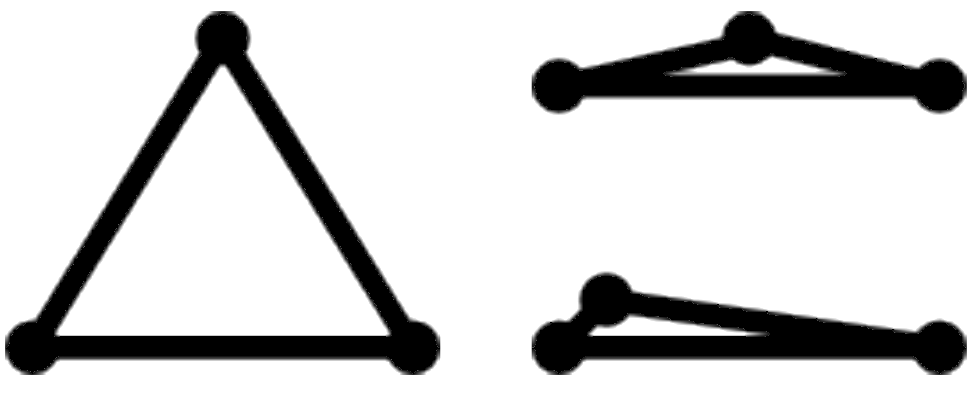
\includegraphics[width=0.7\textwidth]{imagem10}
     \caption{Triângulo bom e triângulos ruins} 
     \label{fig:imagem10}
 \end{figure}

O restante deste trabalho está dividido em quatro seções. No capítulo seguinte faz uma apresentação do que se tem feito atualmente na área de subdivisão de domínios e lá mostraremos mais do método que estamos propondo. O capítulo 3 descreve os algoritmos existentes para geração de malhas bidimensionais, mais precisamente triangulações. Finalmente, no capítulo 4 vamos definir a linha de estudo além do cronograma do trabalho.

